\documentclass[10pt,a4paper]{article}
\usepackage[T1]{fontenc}
\usepackage{lmodern}
\usepackage{amsmath,amssymb,array,booktabs,longtable,tabularx,graphicx,float,placeins}
\usepackage[margin=20mm]{geometry}
\usepackage[unicode,colorlinks=true,linkcolor=blue,urlcolor=blue]{hyperref}
\newcolumntype{P}[1]{>{\raggedright\arraybackslash}p{#1}}
\setlength{\parindent}{0pt}
\setlength{\parskip}{5pt}
\setlength{\emergencystretch}{3em}
\setlength{\tabcolsep}{4pt}
\renewcommand{\arraystretch}{1.18}

% Written to follow Section 2 (small synthetic instance) of numerical_experiments.tex.
% Figures are expected in figures/annual/ (exported from robotaxi_annual.ipynb).
\title{Numerical Experiments: Large case}
\author{}
\date{}
\begin{document}
\maketitle
\setcounter{section}{2}

\section{Large Instance: City-Specific Market Size and Random Choice Probabilities}
\label{sec:annual}
\textbf{Purpose.} Apply the model to an annual instance whose inputs follow the parameter rationale document
(\texttt{4. References/parameter\_rationale\_baseline.tex}): three candidate cities, a fleet of 1{,}000 vehicles, and ten demand scenarios.
The instance is synthetic: the inputs are literature-based proxies, not calibrated data for real cities.
The questions are the same as for the small synthetic instance (Section~2): does the implementation match the formulation, which inputs change the optimal allocation, and where are the switching points.

Two design choices differ from the small instance. First, market size $M_c$ differs across cities (0.75, 1, and 1.25 times the reference value), while all cost and productivity inputs are identical across cities.
Second, the choice probabilities $p_c^s$ are not designed by hand but drawn at random, independently for every city and scenario, from four levels.
The levels $\{0.002,0.005,0.01,0.02\}$ are chosen so that demand and capacity are of the same order of magnitude.
With the reference levels $\{0.02,0.1,0.2,0.4\}$ the smallest scenario demand of any city (11.6 million trips) already exceeded a city's maximum capacity (4.38 million trips); every vehicle then serves $\kappa$ trips wherever it is placed, and any two cities with 500 vehicles each are optimal regardless of $M_c$ and $p_c^s$.
Because $D_c^s=M_cp_c^s$, using levels one tenth as large is identical to scaling every $M_c$ by $0.1$.

\subsection{Baseline Experiment}
\subsubsection{Inputs and Common Settings}
\begin{table}[H]
\centering\small
\caption{Baseline Inputs by City}\label{tab:an-input}
\footnotesize
\begin{tabular}{lP{.30\linewidth}rrrP{.25\linewidth}}
\toprule
Parameter & Definition and unit & A & B & C & Basis (see rationale document)\\\midrule
$M_c$ & Potential trip opportunities (trips/year) & 577{,}908{,}105 & 770{,}544{,}140 & 963{,}180{,}175 & $0.75$, $1$, $1.25\times770{,}544{,}140$ ($=38{,}527{,}207/0.05$); proxy value\\
$\kappa_c$ & Service capacity (trips/vehicle/year) & 8{,}760 & 8{,}760 & 8{,}760 & $24\times365$\\
$\bar q_c$ & City-specific vehicle limit (vehicles) & 500 & 500 & 500 & Assumption\\
$F_c$ & Initial entry cost (USD/city) & 3{,}500{,}000 & 3{,}500{,}000 & 3{,}500{,}000 & $(300{,}000+2{,}500{,}000)\times1.25$\\
$K_c$ & Fixed vehicle cost (USD/vehicle/year) & 7{,}972 & 7{,}972 & 7{,}972 & $4{,}334+1{,}131+1{,}694+813$\\
$c_c^+$ & Unused-capacity penalty (USD/trip) & 0 & 0 & 0 & No additional idle loss (assumption)\\
$c_c^-$ & Forgone contribution margin (USD/trip) & 10 & 10 & 10 & Revenue 18 minus variable cost 8\\
\bottomrule
\end{tabular}
\end{table}
\begin{table}[H]
\centering\small
\caption{Common Settings}\label{tab:an-common}
\begin{tabular}{P{.19\linewidth}P{.72\linewidth}}
\toprule
Item & Setting\\\midrule
$C,Q$ & $C=\{A,B,C\}$, total fleet limit $Q=1{,}000$ vehicles\\
$S$ & $|S|=10$, probability of each scenario $1/|S|=0.1$\\
$p_c^s$ & Drawn independently for each $(c,s)$ from $\{0.002,0.005,0.01,0.02\}$ with equal probability (random seed 2026)\\
$D_c^s$ & $D_c^s=M_cp_c^s$\\
Evaluation period & One year after entry: one-time entry cost plus costs and losses for that year\\
$y_c,q_c$ & Chosen before observing demand and applied to every scenario\\
Operations & No vehicle relocation or capacity sharing across cities; demand in cities not entered is counted as unmet\\
Verification & SciPy MILP (HiGHS) compared with an independent dynamic program over integer vehicle counts, which counts all tied optima; the dynamic program was first checked against full enumeration on the small instance (eight cases, baseline objective 858 reproduced)\\
\bottomrule
\end{tabular}
\end{table}
Each row of Table~\ref{tab:an-scenarios} is one joint demand scenario. Because the levels are drawn independently, a scenario can combine high demand in one city with low demand in another.
\begin{table}[H]
\centering\small
\caption{Random Choice Probabilities and Demand Scenarios (Trips/Year)}\label{tab:an-scenarios}
\begin{tabular}{lrrrrrr}
\toprule
$s$ & $p_A^s$ & $p_B^s$ & $p_C^s$ & $D_A^s$ & $D_B^s$ & $D_C^s$\\\midrule
1 & 0.02 & 0.002 & 0.002 & 11,558,160 & 1,541,088 & 1,926,360\\
2 & 0.01 & 0.005 & 0.005 & 5,779,081 & 3,852,721 & 4,815,901\\
3 & 0.002 & 0.005 & 0.01 & 1,155,816 & 3,852,721 & 9,631,802\\
4 & 0.005 & 0.02 & 0.02 & 2,889,541 & 15,410,883 & 19,263,600\\
5 & 0.01 & 0.02 & 0.01 & 5,779,081 & 15,410,883 & 9,631,802\\
6 & 0.002 & 0.02 & 0.01 & 1,155,816 & 15,410,883 & 9,631,802\\
7 & 0.002 & 0.005 & 0.002 & 1,155,816 & 3,852,721 & 1,926,360\\
8 & 0.02 & 0.01 & 0.02 & 11,558,160 & 7,705,441 & 19,263,600\\
9 & 0.005 & 0.01 & 0.01 & 2,889,541 & 7,705,441 & 9,631,802\\
10 & 0.02 & 0.002 & 0.01 & 11,558,160 & 1,541,088 & 9,631,802\\
Mean & 0.0096 & 0.0099 & 0.0099 & 5,547,917 & 7,628,387 & 9,535,483\\
\bottomrule
\end{tabular}
\end{table}

\subsubsection{Demand Scale versus Capacity}
Before optimizing, compare demand with the capacity a city can deploy at most, $\kappa_c\bar q_c=4{,}380{,}000$ trips. The last column gives the choice probability at which demand equals this capacity.
\begin{table}[H]
\centering\small
\caption{Scenario Demand and Maximum City Capacity (Trips/Year)}\label{tab:an-scale}
\begin{tabular}{lrrrrrr}
\toprule
$c$ & $\min_sD_c^s$ & $\bar D_c$ & $\max_sD_c^s$ & $\kappa_c\bar q_c$ & Scenarios with $D_c^s>\kappa_c\bar q_c$ & $\kappa_c\bar q_c/M_c$\\\midrule
A & 1,155,816 & 5,547,918 & 11,558,162 & 4,380,000 & 5/10 & 0.0076\\
B & 1,541,088 & 7,628,387 & 15,410,883 & 4,380,000 & 5/10 & 0.0057\\
C & 1,926,360 & 9,535,484 & 19,263,604 & 4,380,000 & 8/10 & 0.0045\\
\bottomrule
\end{tabular}
\end{table}
\begin{figure}[H]
\centering
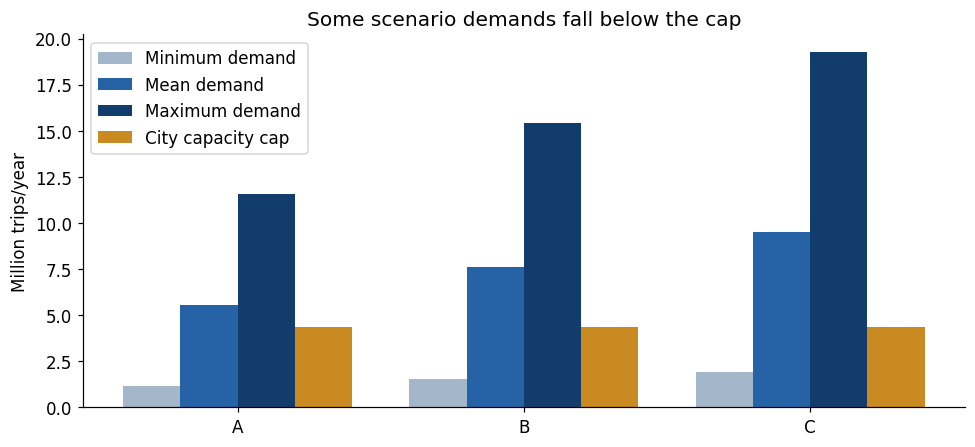
\includegraphics[width=.8\linewidth]{figures/annual/01_scale.png}
\caption{Minimum, mean, and maximum scenario demand compared with the maximum city capacity.}\label{fig:an-01_scale}
\end{figure}
\textbf{Interpretation.} Demand straddles capacity: in half of the scenarios for A and B, and in eight of ten for C, demand exceeds what 500 vehicles can serve, while in the remaining scenarios part of the capacity would be idle.
This is the regime in which the allocation depends on demand. Meeting mean demand in every city would require 2{,}593 vehicles against a fleet of 1{,}000.

\FloatBarrier
\subsubsection{Optimal Allocation and Cost}
The optimal solution enters all three cities. The representative allocation is $q=(132,368,500)$, but it is not unique: 72 allocations share the same objective. In all of them $q_A=132$, while $q_B$ ranges from 368 to 439 and $q_C$ from 429 to 500 with $q_B+q_C=868$.
All checks passed: integrality, nonnegativity, city-specific and total fleet limits, demand--capacity balance, objective recalculation, and agreement between the MILP and the dynamic program.
\begin{table}[H]
\centering\small
\caption{City-Level Results for the Representative Optimum (Trips/Year)}\label{tab:an-base-city}
\begin{tabular}{lrrrrrrr}
\toprule
$c$ & $y_c$ & $q_c$ & $\kappa_cq_c$ & $\bar D_c$ & $\bar T_c$ & $\bar U_c$ & $\bar O_c$\\\midrule
A & 1 & 132 & 1,156,320 & 5,547,918 & 1,156,169 & 4,391,749 & 151\\
B & 1 & 368 & 3,223,680 & 7,628,387 & 2,887,162 & 4,741,225 & 336,518\\
C & 1 & 500 & 4,380,000 & 9,535,484 & 3,889,272 & 5,646,212 & 490,728\\
Total & 3 & 1000 & 8,760,000 & 22,711,789 & 7,932,603 & 14,779,186 & 827,397\\
\bottomrule
\end{tabular}
\end{table}
\begin{table}[H]
\centering\small
\caption{Baseline Cost Breakdown and Performance (USD)}\label{tab:an-base-cost}
\begin{tabular}{rrrrrrr}
\toprule
$C_F$ & $C_K$ & $C_O$ & $C_U$ & $Z$ & $Z_0$ & $\Delta Z$\\\midrule
10,500,000 & 7,972,000 & 0 & 147,791,859 & 166,263,859 & 227,117,885 & 60,854,026\\
\bottomrule
\end{tabular}
\end{table}
The service rate is $\mathrm{SR}=34.93\%$ and capacity utilization is $\mathrm{CU}=90.55\%$.
On average 827{,}397 trips of capacity are unused, almost all of it in B and C: in the scenarios where their demand is at the lowest level, the deployed capacity exceeds demand. Subtracting entry costs of 10.5 million and vehicle costs of 7.97 million from the service contribution of $7{,}932{,}603\times10=79.3$ million gives an improvement of 60.85 million.
\begin{table}[H]
\centering\small
\caption{Scenario Totals for Allocation $(132,368,500)$ (Trips/Year)}\label{tab:an-scenario-result}
\begin{tabular}{lrrrr}
\toprule
$s$ & $\sum_cD_c^s$ & $\sum_cT_c^s$ & $\sum_cU_c^s$ & $\sum_cO_c^s$\\\midrule
1 & 15,025,610 & 4,623,769 & 10,401,840 & 4,136,231\\
2 & 14,447,700 & 8,760,000 & 5,687,703 & 0\\
3 & 14,640,340 & 8,759,496 & 5,880,842 & 504\\
4 & 37,564,030 & 8,760,000 & 28,804,030 & 0\\
5 & 30,821,770 & 8,760,000 & 22,061,770 & 0\\
6 & 26,198,500 & 8,759,496 & 17,439,000 & 504\\
7 & 6,934,897 & 6,305,857 & 629,041 & 2,454,143\\
8 & 38,527,210 & 8,760,000 & 29,767,210 & 0\\
9 & 20,226,780 & 8,760,000 & 11,466,780 & 0\\
10 & 22,731,050 & 7,077,408 & 15,653,640 & 1,682,592\\
Mean & 22,711,789 & 7,932,603 & 14,779,186 & 827,397\\
\bottomrule
\end{tabular}
\end{table}
\begin{figure}[H]
\centering
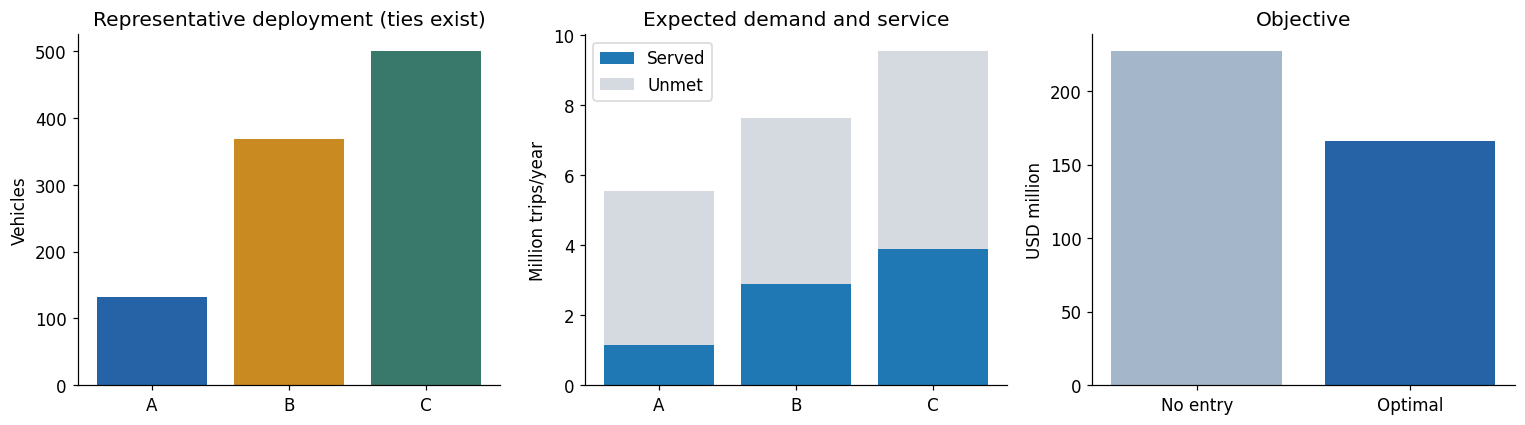
\includegraphics[width=\linewidth]{figures/annual/02_baseline.png}
\caption{Representative allocation, expected served and unmet demand by city, and the objective compared with no entry.}\label{fig:an-02_baseline}
\end{figure}

\FloatBarrier
\subsubsection{Why 132 Vehicles in A, and Why B and C Tie}
The allocation can be read from the value of one additional vehicle. A vehicle adds $\kappa=8{,}760$ trips of capacity and costs $K=7{,}972$.
In a scenario where demand still exceeds capacity, it serves 8{,}760 more trips and avoids $8{,}760\times10=87{,}600$ of forgone margin; in a scenario where demand is already fully served it adds nothing, because $c^+=0$.
The expected value of one more vehicle is therefore
\[
87{,}600\times\bigl(\text{share of scenarios with unmet demand}\bigr)-7{,}972 .
\]
As vehicles are added to a city, the low-demand scenarios become fully served one after another and this value steps down (Table~\ref{tab:an-ladder}).
\begin{table}[H]
\centering\small
\caption{Value of the $k$-th Vehicle in Each City (USD/Year)}\label{tab:an-ladder}
\begin{tabular}{llll}
\toprule
$c$ & Vehicle $k$ & Scenarios with unmet demand & Value of vehicle $k$\\\midrule
A & 1--131 & 10/10 & 79,628\\
A & 132 & boundary & 78,117\\
A & 133--329 & 7/10 & 53,348\\
A & 330 & boundary & 50,829\\
A & 331--500 & 5/10 & 35,828\\
B & 1--175 & 10/10 & 79,628\\
B & 176 & boundary & 78,285\\
B & 177--439 & 8/10 & 62,108\\
B & 440 & boundary & 57,070\\
B & 441--500 & 5/10 & 35,828\\
C & 1--219 & 10/10 & 79,628\\
C & 220 & boundary & 77,949\\
C & 221--500 & 8/10 & 62,108\\
\bottomrule
\end{tabular}
\end{table}
The optimizer fills the most valuable slots first: A's first 132, B's first 176, and C's first 220 vehicles, 528 in total, each worth 77{,}949 or more.
The remaining 472 vehicles go to the slots worth 62{,}108, B's 177th--439th and C's 221st--500th; these 543 slots have identical value, so any split of the 472 vehicles between B and C is optimal.
This produces the 72 tied allocations. A's next vehicle is worth 53{,}348, less than 62{,}108, so A stays at 132.
The ties are a consequence of ten equally likely scenarios: the value of a vehicle moves in steps of one tenth, and B and C sit on the same step over a wide range of vehicle counts.

Entering A is worthwhile, but only narrowly. Table~\ref{tab:an-plans} compares the optimum with other allocations of 1{,}000 vehicles.
A's 132 vehicles contribute 10.51 million before entry cost; the entry cost is 3.5 million; and the same 132 vehicles placed in B (its 369th--500th, of which 60 serve only five scenarios) would contribute 6.62 million. The net advantage of entering A is $10.51-3.50-6.62=0.39$ million.
This margin determines the switching points in Section~\ref{sec:an-sens}.
\begin{table}[H]
\centering\small
\caption{Comparison of Allocations Using 1{,}000 Vehicles (Costs in USD Million)}\label{tab:an-plans}
\begin{tabular}{lrrrrrr}
\toprule
$q$ & $\bar T$ (trips) & $C_F$ & $C_K$ & $C_U$ & $Z$ & $\Delta Z$\\\midrule
$(132,368,500)$ & 7,932,603 & 10.50 & 7.97 & 147.79 & 166.26 & 60.85\\
$(132,439,429)$ & 7,932,603 & 10.50 & 7.97 & 147.79 & 166.26 & 60.85\\
$(0,500,500)$ & 7,543,306 & 7.00 & 7.97 & 151.68 & 166.66 & 60.46\\
$(334,333,333)$ & 7,748,391 & 10.50 & 7.97 & 149.63 & 168.11 & 59.01\\
$(500,250,250)$ & 7,312,143 & 10.50 & 7.97 & 154.00 & 172.47 & 54.65\\
$(500,0,500)$ & 7,003,925 & 7.00 & 7.97 & 157.08 & 172.05 & 55.07\\
$(500,500,0)$ & 6,768,687 & 7.00 & 7.97 & 159.43 & 174.40 & 52.71\\
\bottomrule
\end{tabular}
\end{table}
\textbf{Interpretation.} The first two rows are two of the 72 tied optima. Leaving A out costs 0.39 million; an even split across cities costs 1.84 million more than the optimum because it moves vehicles from B and C's 62{,}108-valued slots into A's 53{,}348- and 35{,}828-valued slots.
Concentrating in two cities without C is worst: C has the largest market and the fewest low-demand scenarios.

\FloatBarrier
\subsection{Edge-Case Experiments}
Each experiment changes only the listed input relative to the baseline. Because the expected properties of the small instance were tied to its numbers, the checks here are stated as properties that hold regardless of input scale (no entry, local optimality, or bounds on the improvement).
\begin{table}[H]
\centering\small
\caption{Modified Inputs and Expected Properties for Edge Cases}\label{tab:an-edge-design}
\begin{tabular}{lP{.36\linewidth}P{.50\linewidth}}
\toprule
Case & Modified input & Expected property\\\midrule
E1 & $Q=0$ & $y=q=0$; $U_c^s=D_c^s$\\
E2 & $M=(0,0,0)$ & $y=q=0$; $Z=0$, $U_c^s=O_c^s=0$\\
E3 & $\bar q=(0,500,500)$ & $y_A=q_A=0$; B, C locally optimal\\
E4 & $c^-=(0,0,0)$ & No service incentive: $y=q=0$, $Z=0$\\
E5 & $F_c=Z_0+1$ for all $c$ & Entry cost above total service value: $y=q=0$\\
E6 & $Q=2{,}000$ & Fleet limit not binding: $\sum_cq_c\le1{,}500$, $\Delta Z\ge$ baseline\\
E7 & $F=(0,0,0)$ & $\Delta Z\ge$ baseline; $\sum_cq_c\le Q$\\
E8 & $p_c^s=\kappa_c/M_c$ ($\forall c,s$), $F=0$ & $D_c^s=8{,}760$; $q=(1,1,1)$; $U_c^s=O_c^s=0$\\
\bottomrule
\end{tabular}
\end{table}
\begin{table}[H]
\centering\small
\caption{Allocation and Service Results for Edge Cases (Trips/Year)}\label{tab:an-edge-service}
\begin{tabular}{lrrrrrrr}
\toprule
Case & $q^{\mathrm{rep}}$ & Ties & $\bar T$ & $\mathrm{SR}$ (\%) & $\bar U$ & $\bar O$ & Check\\\midrule
E1 & $(0,0,0)$ & 1 & 0 & 0.00 & 22,711,790 & 0 & PASS\\
E2 & $(0,0,0)$ & 1 & 0 & --- & 0 & 0 & PASS\\
E3 & $(0,500,500)$ & 1 & 7,543,306 & 33.21 & 15,168,480 & 1,216,694 & PASS\\
E4 & $(0,0,0)$ & 1 & 0 & 0.00 & 22,711,790 & 0 & PASS\\
E5 & $(0,0,0)$ & 1 & 0 & 0.00 & 22,711,790 & 0 & PASS\\
E6 & $(500,500,500)$ & 1 & 10,657,960 & 46.93 & 12,053,830 & 2,482,041 & PASS\\
E7 & $(132,368,500)$ & 72 & 7,932,603 & 34.93 & 14,779,190 & 827,397 & PASS\\
E8 & $(1,1,1)$ & 1 & 26,280 & 100.00 & 0 & 0 & PASS\\
\bottomrule
\end{tabular}
\end{table}
\begin{table}[H]
\centering\small
\caption{Edge-Case Cost Breakdown and Improvement (USD Million)}\label{tab:an-edge-cost}
\begin{tabular}{lrrrrrrr}
\toprule
Case & $C_F$ & $C_K$ & $C_O$ & $C_U$ & $Z$ & $Z_0$ & $\Delta Z$\\\midrule
E1 & 0.00 & 0.00 & 0.00 & 227.12 & 227.12 & 227.12 & 0.00\\
E2 & 0.00 & 0.00 & 0.00 & 0.00 & 0.00 & 0.00 & 0.00\\
E3 & 7.00 & 7.97 & 0.00 & 151.68 & 166.66 & 227.12 & 60.46\\
E4 & 0.00 & 0.00 & 0.00 & 0.00 & 0.00 & 0.00 & 0.00\\
E5 & 0.00 & 0.00 & 0.00 & 227.12 & 227.12 & 227.12 & 0.00\\
E6 & 10.50 & 11.96 & 0.00 & 120.54 & 143.00 & 227.12 & 84.12\\
E7 & 0.00 & 7.97 & 0.00 & 147.79 & 155.76 & 227.12 & 71.35\\
E8 & 0.00 & 0.02 & 0.00 & 0.00 & 0.02 & 0.26 & 0.24\\
\bottomrule
\end{tabular}
\end{table}
\begin{figure}[H]
\centering
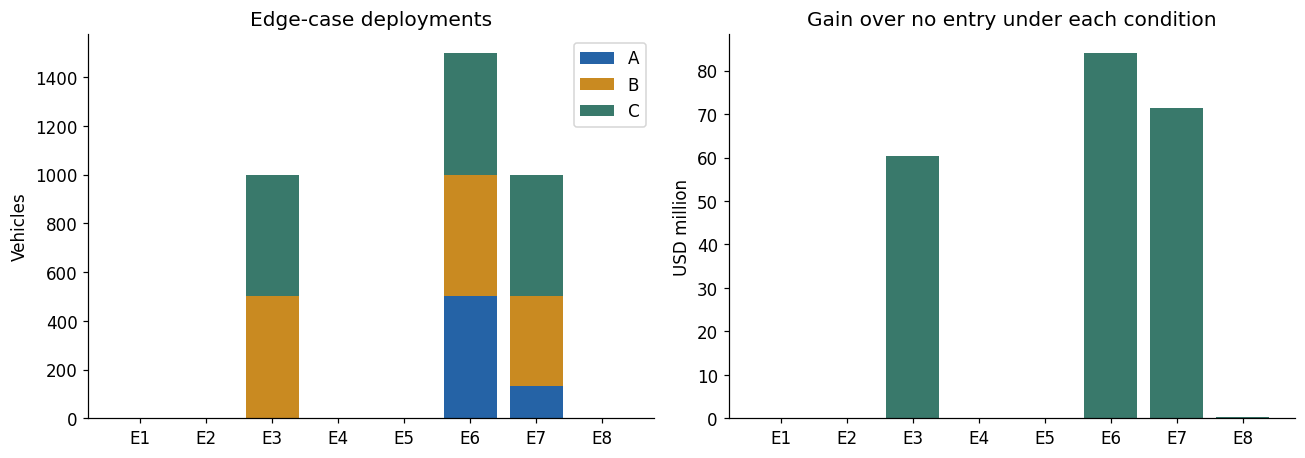
\includegraphics[width=\linewidth]{figures/annual/03_edges.png}
\caption{Allocations and improvements for E1--E8. Objectives under different conditions do not constitute a performance ranking.}\label{fig:an-03_edges}
\end{figure}
\textbf{Interpretation.} E1, E4, and E5 result in no entry; E4 has a zero objective because unmet demand carries no loss.
E3 (A cannot be entered) loses exactly the 0.39 million value of entering A. E6 relaxes the fleet limit and deploys 1{,}500 vehicles, the sum of the city limits, raising the improvement to 84.12 million.
E7 removes entry costs but keeps the allocation, because the fleet limit, not the entry cost, caps A at 132 vehicles; the improvement rises by exactly $3F=10.5$ million.
E8 sets demand equal to one vehicle's capacity in every scenario and serves it exactly with one vehicle per city.

\FloatBarrier
\subsection{Sensitivity Analysis}\label{sec:an-sens}
\subsubsection{Experimental Design and Interpretation}
One input type is varied at a time, with all other inputs fixed at their baseline values, and the model is reoptimized.
Common-level experiments change the input in all cities at once; the $M_A$ experiment changes only A, and Section~\ref{sec:an-city} changes one input in one city at a time.
\begin{table}[H]
\centering\small
\caption{Parameter Ranges for the Sensitivity Experiments}\label{tab:an-sens-design}
\begin{tabular}{lP{.50\linewidth}P{.30\linewidth}}
\toprule
Parameter & Variation and range & Note\\\midrule
$Q$ & Total fleet limit: 0--2{,}000, step 100 & $\bar q_c=500$\\
$F$ & Common across cities: $\pm25\%$ of 3.5 million, 9 points & \\
$K$ & Common across cities: $\pm25\%$ of 7{,}972, 9 points & \\
$\kappa$ & Common across cities: $\pm25\%$ of 8{,}760, 9 points & \\
$M$ multiplier & All cities scaled by 0.75--1.25, 9 points; city ratios 0.75:1:1.25 kept & Identical to scaling all $p_c^s$\\
$p$ multiplier & All $p_c^s$ scaled by 0.75, 1, 1.25 & Identical to the $M$ multiplier\\
$\bar q$ & Common city limit: 100, 250, 500, 750, 1{,}000, 1{,}500 & $Q=1{,}000$\\
$c^+$ & Common across cities: 0, 1, 3, 5, 10, 15, 40 & Baseline 0\\
$c^-$ & Common across cities: 2, 5, 10, 15, 20 & \\
$M_A$ & A only: 0.75--1.25 times baseline, 9 points & $M_B,M_C$ fixed\\
$\alpha$ & Demand variability multiplier $p_c^s(\alpha)=\bar p_c+\alpha(p_c^s-\bar p_c)$: 0--1, step 0.1 & City mean demands unchanged\\
\bottomrule
\end{tabular}
\end{table}
Read the panels of each figure in the order allocation, service rate, cost breakdown, and improvement. Shaded bands show the range of each city's vehicle count across tied optimal solutions, not confidence intervals; they are drawn only at the grid points.
The representative solution minimizes the number of entered cities first and then uses lexicographic order on $q$.
Switching points are located only between adjacent grid values unless a closed-form comparison is available. In the tables, $\bar T$ is in trips/year and $Z$, $\Delta Z$ in USD million.

\subsubsection{Total Fleet Limit $Q$}
\begin{table}[H]
\centering\small
\caption{Selected Results: Total Fleet Limit}\label{tab:an-selected-Q}
\begin{tabular}{lrrrrrr}
\toprule
Value & $q^{\mathrm{rep}}$ & Ties & $\bar T$ & $\mathrm{SR}$ (\%) & $Z$ & $\Delta Z$\\\midrule
0 & $(0,0,0)$ & 1 & 0 & 0.00 & 227.12 & 0.00\\
100 & $(0,0,100)$ & 3 & 876,000 & 3.86 & 222.66 & 4.46\\
300 & $(0,0,300)$ & 1 & 2,487,672 & 10.95 & 208.13 & 18.99\\
500 & $(0,0,500)$ & 1 & 3,889,272 & 17.12 & 195.71 & 31.41\\
600 & $(0,176,424)$ & 205 & 4,898,290 & 21.57 & 189.92 & 37.20\\
800 & $(0,300,500)$ & 140 & 6,299,890 & 27.74 & 177.50 & 49.62\\
900 & $(0,400,500)$ & 40 & 7,000,690 & 30.82 & 171.29 & 55.83\\
1,000 & $(132,368,500)$ & 72 & 7,932,603 & 34.93 & 166.26 & 60.85\\
1,100 & $(160,440,500)$ & 1 & 8,608,371 & 37.90 & 160.30 & 66.81\\
1,200 & $(260,440,500)$ & 1 & 9,221,571 & 40.60 & 154.97 & 72.15\\
1,300 & $(330,470,500)$ & 31 & 9,781,959 & 43.07 & 150.16 & 76.96\\
1,400 & $(400,500,500)$ & 61 & 10,219,959 & 45.00 & 146.58 & 80.54\\
1,500 & $(500,500,500)$ & 1 & 10,657,959 & 46.93 & 143.00 & 84.12\\
2,000 & $(500,500,500)$ & 1 & 10,657,959 & 46.93 & 143.00 & 84.12\\
\bottomrule
\end{tabular}
\end{table}
\begin{figure}[H]
\centering
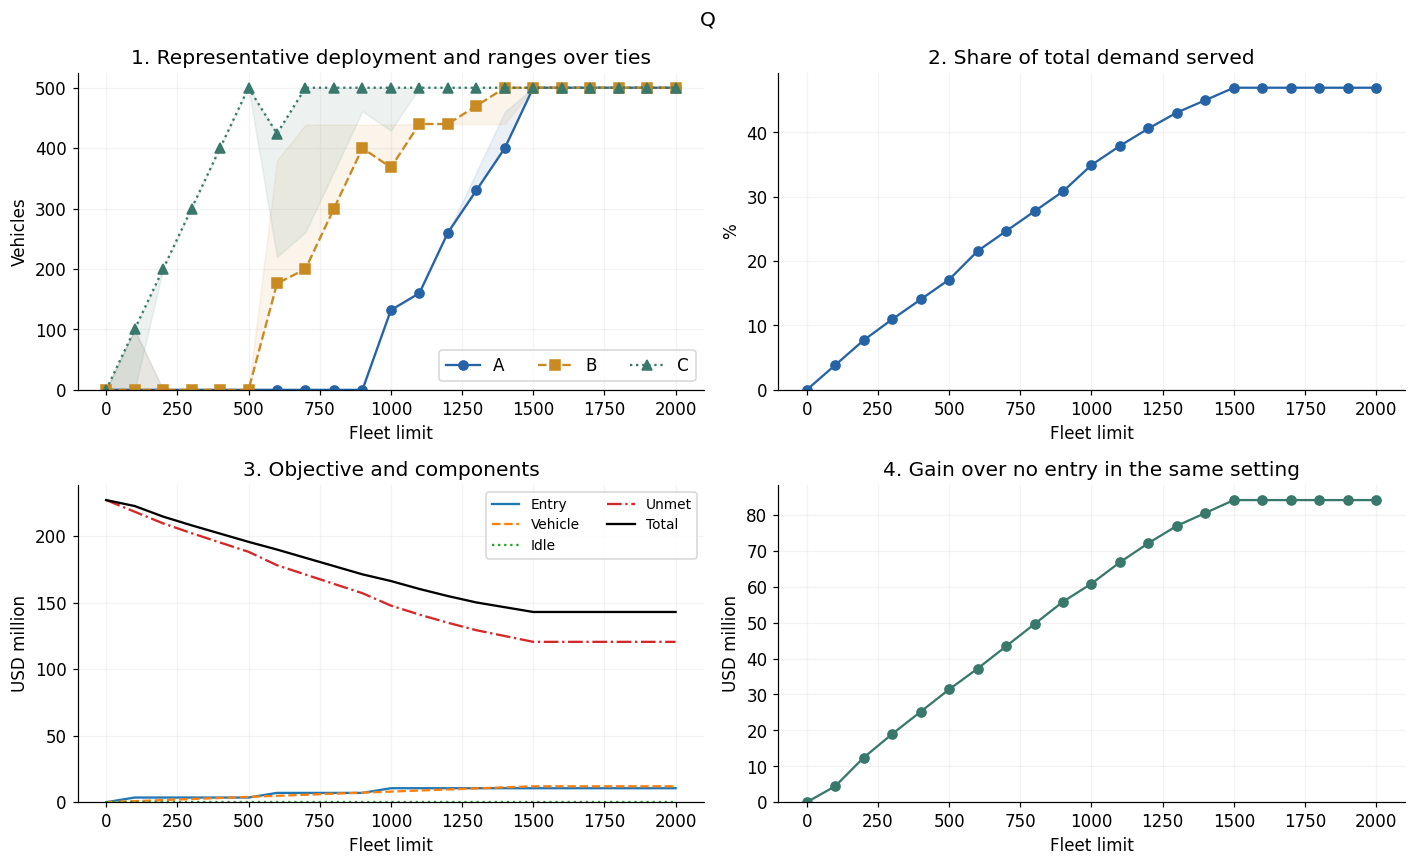
\includegraphics[width=\linewidth]{figures/annual/sweep_Q.png}
\caption{Allocation, service rate, cost, and improvement as the total fleet limit varies.}\label{fig:an-sweep_Q}
\end{figure}
\textbf{Interpretation.} Up to 500 vehicles, everything goes to a single city, C, because a second entry cost is not yet worth paying (at $Q=100$ any one city would do).
From 600 vehicles B is entered and B and C share the fleet with many ties. A is entered only at $Q\ge1{,}000$, and from 1{,}100 its fleet grows quickly because its next slots (53{,}348 and 35{,}828) are now the best remaining. At $Q\ge1{,}500$ the city limits bind and the results stop changing.

\clearpage
\subsubsection{Common Entry Cost $F$}
\begin{table}[H]
\centering\small
\caption{Selected Results: Common Entry Cost}\label{tab:an-selected-F}
\begin{tabular}{lrrrrrr}
\toprule
Value & $q^{\mathrm{rep}}$ & Ties & $\bar T$ & $\mathrm{SR}$ (\%) & $Z$ & $\Delta Z$\\\midrule
2,625,000 & $(132,368,500)$ & 72 & 7,932,603 & 34.93 & 163.64 & 63.48\\
2,843,750 & $(132,368,500)$ & 72 & 7,932,603 & 34.93 & 164.30 & 62.82\\
3,062,500 & $(132,368,500)$ & 72 & 7,932,603 & 34.93 & 164.95 & 62.17\\
3,281,250 & $(132,368,500)$ & 72 & 7,932,603 & 34.93 & 165.61 & 61.51\\
3,500,000 & $(132,368,500)$ & 72 & 7,932,603 & 34.93 & 166.26 & 60.85\\
3,718,750 & $(132,368,500)$ & 72 & 7,932,603 & 34.93 & 166.92 & 60.20\\
3,937,500 & $(0,500,500)$ & 1 & 7,543,306 & 33.21 & 167.53 & 59.59\\
4,156,250 & $(0,500,500)$ & 1 & 7,543,306 & 33.21 & 167.97 & 59.15\\
4,375,000 & $(0,500,500)$ & 1 & 7,543,306 & 33.21 & 168.41 & 58.71\\
\bottomrule
\end{tabular}
\end{table}
\begin{figure}[H]
\centering
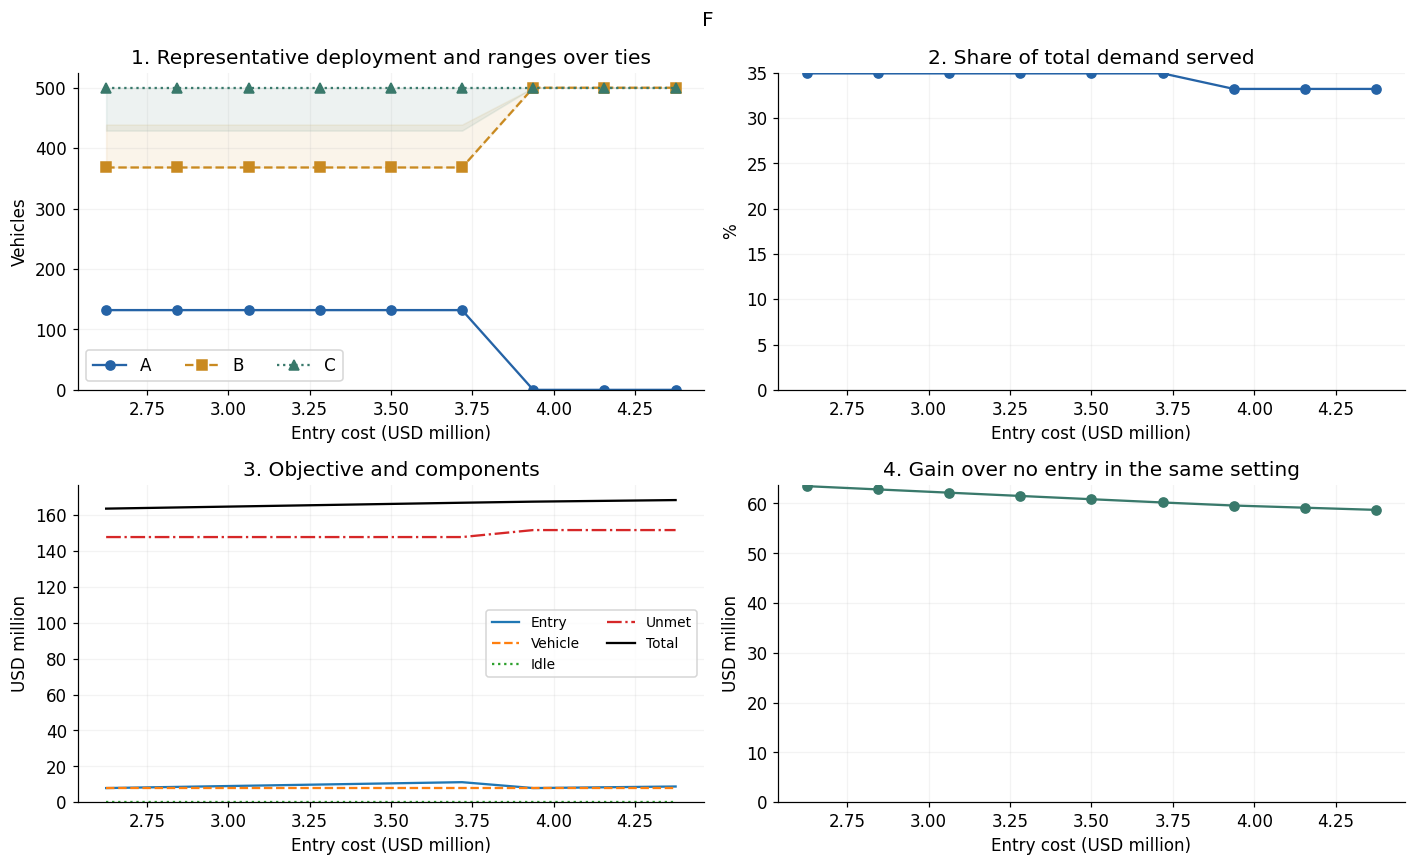
\includegraphics[width=\linewidth]{figures/annual/sweep_F.png}
\caption{Results from varying the common entry cost within $\pm25\%$.}\label{fig:an-sweep_F}
\end{figure}
\textbf{Interpretation.} The entry cost changes only whether A is entered. The three-city allocation beats $(0,500,500)$ by 0.39 million at $F=3.5$ million, and both alternatives pay $F$ for B and C, so the two tie at $F=3{,}500{,}000+392{,}967=3{,}892{,}967$; A is dropped at the next grid point, 3.94 million.
Within each regime $\Delta Z$ falls linearly with $F$ (slope $-3$ with three cities, $-2$ with two).

\clearpage
\subsubsection{Common Vehicle Cost $K$}
\begin{table}[H]
\centering\small
\caption{Selected Results: Common Vehicle Cost}\label{tab:an-selected-K}
\begin{tabular}{lrrrrrr}
\toprule
Value & $q^{\mathrm{rep}}$ & Ties & $\bar T$ & $\mathrm{SR}$ (\%) & $Z$ & $\Delta Z$\\\midrule
5,979.0 & $(132,368,500)$ & 72 & 7,932,603 & 34.93 & 164.27 & 62.85\\
6,975.5 & $(132,368,500)$ & 72 & 7,932,603 & 34.93 & 165.27 & 61.85\\
7,972.0 & $(132,368,500)$ & 72 & 7,932,603 & 34.93 & 166.26 & 60.85\\
8,968.5 & $(132,368,500)$ & 72 & 7,932,603 & 34.93 & 167.26 & 59.86\\
9,965.0 & $(132,368,500)$ & 72 & 7,932,603 & 34.93 & 168.26 & 58.86\\
\bottomrule
\end{tabular}
\end{table}
\textbf{Interpretation.} Within $\pm25\%$ the allocation does not change: the fleet limit binds, all 1{,}000 vehicles are used, and a common $K$ lowers every vehicle's value by the same amount. Only the improvement changes, by $-1{,}000$ USD per USD of $K$.

\subsubsection{Vehicle Productivity $\kappa$}
\begin{table}[H]
\centering\small
\caption{Selected Results: Vehicle Productivity}\label{tab:an-selected-kappa}
\begin{tabular}{lrrrrrr}
\toprule
Value & $q^{\mathrm{rep}}$ & Ties & $\bar T$ & $\mathrm{SR}$ (\%) & $Z$ & $\Delta Z$\\\midrule
6,570.0 & $(0,500,500)$ & 1 & 5,949,490 & 26.20 & 182.59 & 44.52\\
7,117.5 & $(0,500,500)$ & 1 & 6,387,490 & 28.12 & 178.21 & 48.90\\
7,665.0 & $(0,500,500)$ & 1 & 6,825,490 & 30.05 & 173.83 & 53.28\\
8,212.5 & $(0,500,500)$ & 1 & 7,187,431 & 31.65 & 170.22 & 56.90\\
8,760.0 & $(132,368,500)$ & 72 & 7,932,603 & 34.93 & 166.26 & 60.85\\
9,307.5 & $(124,376,500)$ & 38 & 8,370,316 & 36.85 & 161.89 & 65.23\\
9,855.0 & $(118,391,491)$ & 3 & 8,805,480 & 38.77 & 157.54 & 69.58\\
10,402.5 & $(130,370,500)$ & 38 & 9,188,467 & 40.46 & 153.71 & 73.41\\
10,950.0 & $(148,352,500)$ & 61 & 9,571,761 & 42.14 & 149.87 & 77.25\\
\bottomrule
\end{tabular}
\end{table}
\begin{figure}[H]
\centering
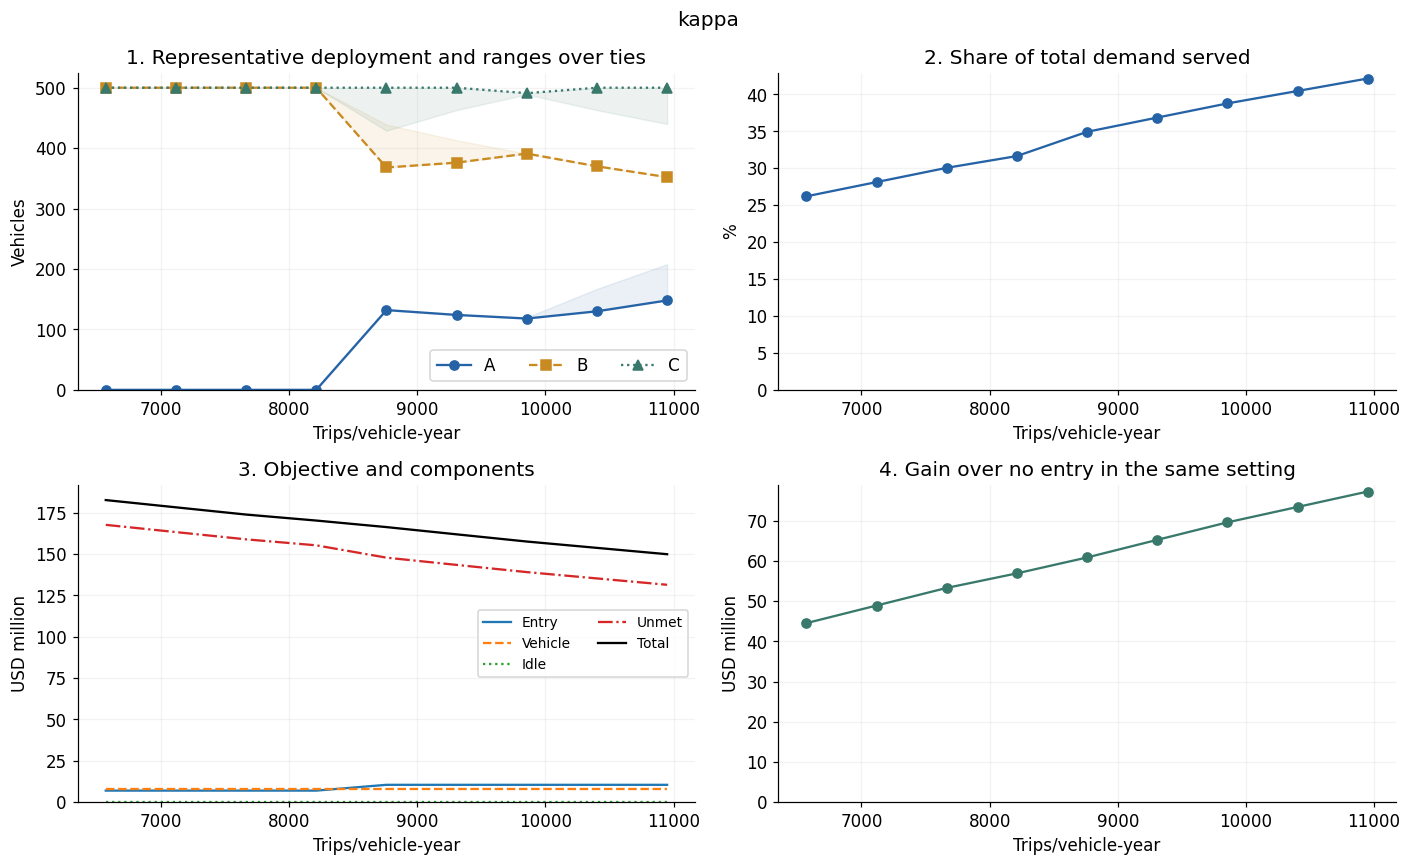
\includegraphics[width=\linewidth]{figures/annual/sweep_kappa.png}
\caption{Results from varying service capacity per vehicle.}\label{fig:an-sweep_kappa}
\end{figure}
\textbf{Interpretation.} Lower productivity removes A: at $\kappa\le8{,}212.5$ the optimum is $(0,500,500)$. Two effects work against A. A's vehicles are used in all ten scenarios, so each loses 10 USD per trip of lost capacity, whereas the B vehicles they displace are used in eight or five scenarios and lose less.
In addition, more vehicles are needed to cover B's 3.85-million scenarios, so B's cheap tail (vehicles serving only five scenarios) shrinks and the displaced vehicles become more valuable.
The switch lies between 8{,}212.5 and 8{,}760; bisection on the same model places it near $\kappa\approx8{,}498$. Higher productivity keeps three cities and raises the improvement by 3.8--4.4 million per grid step (6.25\% of $\kappa$).

\clearpage
\subsubsection{Market Size and Choice Probability Multipliers}
Scaling all $M_c$ and scaling all $p_c^s$ by the same factor give identical results because only $D_c^s=M_cp_c^s$ enters the model; the $p$-multiplier points $0.75$, $1$, $1.25$ coincide with the corresponding rows below.
\begin{table}[H]
\centering\small
\caption{Selected Results: Common Multiplier on $M_c$ (City Ratios Kept)}\label{tab:an-selected-M}
\begin{tabular}{lrrrrrr}
\toprule
Value & $q^{\mathrm{rep}}$ & Ties & $\bar T$ & $\mathrm{SR}$ (\%) & $Z$ & $\Delta Z$\\\midrule
0.7500 & $(170,330,500)$ & 78 & 7,562,071 & 44.39 & 113.19 & 57.15\\
0.8125 & $(143,357,500)$ & 54 & 7,681,215 & 41.63 & 126.19 & 58.34\\
0.8750 & $(116,385,499)$ & 18 & 7,800,416 & 39.25 & 139.20 & 59.53\\
0.9375 & $(124,376,500)$ & 37 & 7,874,596 & 36.98 & 152.65 & 60.27\\
1.0000 & $(132,368,500)$ & 72 & 7,932,603 & 34.93 & 166.26 & 60.85\\
1.0625 & $(0,500,500)$ & 1 & 7,658,888 & 31.74 & 179.70 & 61.62\\
1.1250 & $(0,500,500)$ & 1 & 7,774,469 & 30.43 & 192.73 & 62.77\\
1.1875 & $(0,500,500)$ & 1 & 7,831,519 & 29.04 & 206.36 & 63.34\\
1.2500 & $(0,500,500)$ & 1 & 7,874,862 & 27.74 & 220.12 & 63.78\\
\bottomrule
\end{tabular}
\end{table}
\begin{figure}[H]
\centering
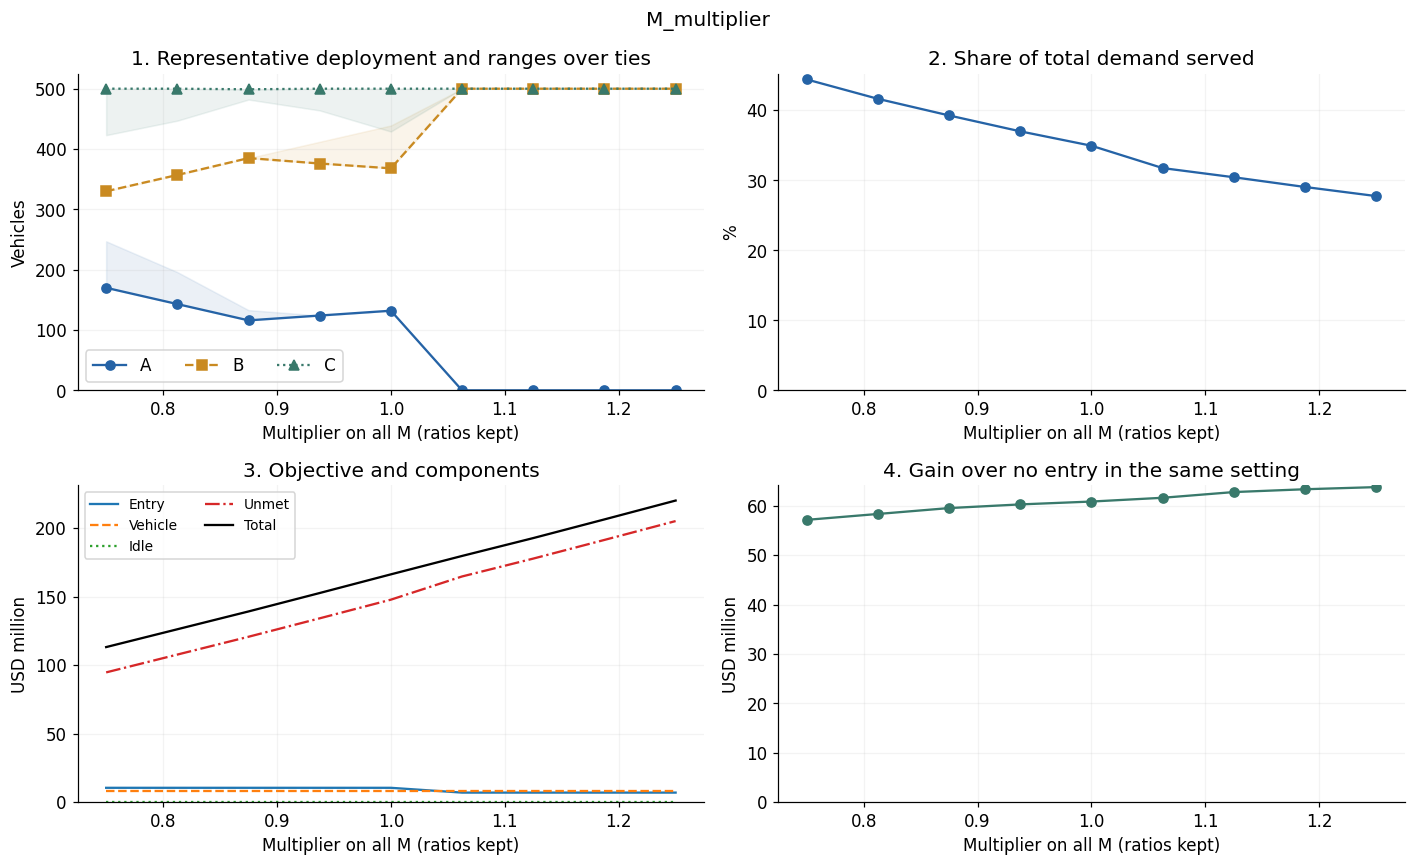
\includegraphics[width=\linewidth]{figures/annual/sweep_M_multiplier.png}
\caption{Results from scaling all market sizes with city ratios kept.}\label{fig:an-sweep_M}
\end{figure}
\textbf{Interpretation.} Smaller demand keeps three cities and moves vehicles into A (170 at $0.75$), because B and C reach their fully served scenarios with fewer vehicles.
Larger demand drops A from $1.0625$ on: B's cheap tail shrinks as its 3.85-million scenarios grow, so the vehicles A would displace are worth more than A's entry. The switch lies between $1$ and $1.0625$ (bisection: about $1.042$).
Note that $Z$ rises with demand even though the improvement rises: the no-entry benchmark $Z_0$ grows with demand, so $Z$ alone does not rank performance.

\clearpage
\subsubsection{City Vehicle Limit $\bar q$}
\begin{table}[H]
\centering\small
\caption{Selected Results: Common City Vehicle Limit}\label{tab:an-selected-qbar}
\begin{tabular}{lrrrrrr}
\toprule
Value & $q^{\mathrm{rep}}$ & Ties & $\bar T$ & $\mathrm{SR}$ (\%) & $Z$ & $\Delta Z$\\\midrule
100 & $(100,100,100)$ & 1 & 2,628,000 & 11.57 & 213.73 & 13.39\\
250 & $(250,250,250)$ & 1 & 6,077,235 & 26.76 & 182.82 & 44.29\\
500 & $(132,368,500)$ & 72 & 7,932,603 & 34.93 & 166.26 & 60.85\\
750 & $(0,440,560)$ & 1 & 7,692,016 & 33.87 & 165.17 & 61.95\\
1,000 & $(0,440,560)$ & 1 & 7,692,016 & 33.87 & 165.17 & 61.95\\
1,500 & $(0,440,560)$ & 1 & 7,692,016 & 33.87 & 165.17 & 61.95\\
\bottomrule
\end{tabular}
\end{table}
\begin{figure}[H]
\centering
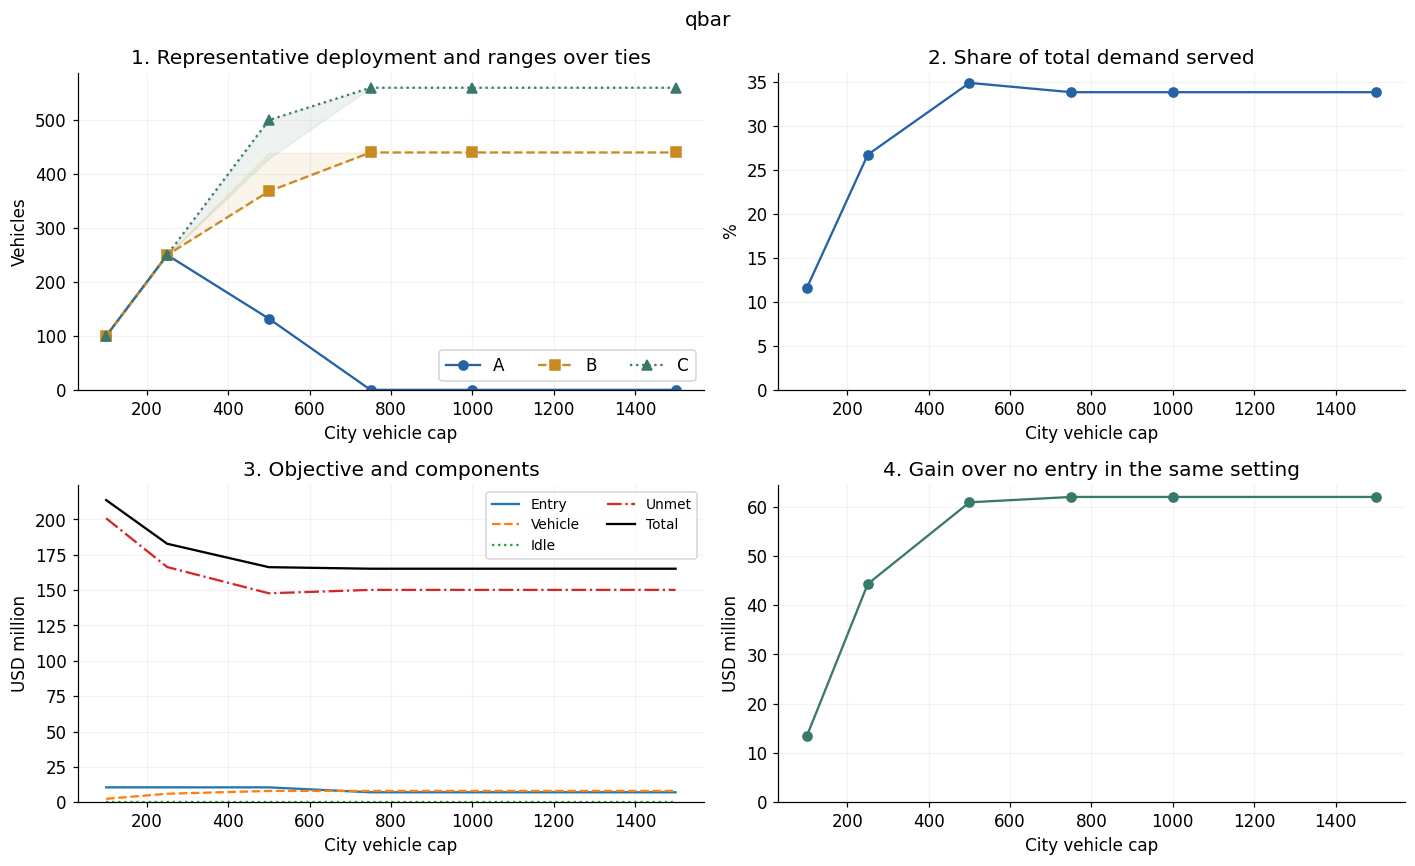
\includegraphics[width=\linewidth]{figures/annual/sweep_qbar.png}
\caption{Results from varying the city-specific vehicle limit with $Q=1{,}000$.}\label{fig:an-sweep_qbar}
\end{figure}
\textbf{Interpretation.} A tight limit forces an even split; at 100 and 250 every city receives its limit. From 750 upward the optimum is $(0,440,560)$ and stops changing: C takes 560 vehicles (capacity 4.91 million, just above its 4.82-million scenario), B stops at 440 where its next vehicles would serve only five scenarios, and the extra room in C is worth more than entering A.

\clearpage
\subsubsection{Common Unused-Capacity Penalty $c^+$}
\begin{table}[H]
\centering\small
\caption{Selected Results: Common Unused-Capacity Penalty}\label{tab:an-selected-cplus}
\begin{tabular}{lrrrrrr}
\toprule
Value & $q^{\mathrm{rep}}$ & Ties & $\bar T$ & $\mathrm{SR}$ (\%) & $Z$ & $\Delta Z$\\\midrule
0 & $(132,368,500)$ & 72 & 7,932,603 & 34.93 & 166.26 & 60.85\\
1 & $(132,368,500)$ & 72 & 7,932,603 & 34.93 & 167.09 & 60.03\\
3 & $(132,368,500)$ & 72 & 7,932,603 & 34.93 & 168.75 & 58.37\\
5 & $(132,368,500)$ & 72 & 7,932,603 & 34.93 & 170.40 & 56.72\\
10 & $(132,368,500)$ & 72 & 7,932,603 & 34.93 & 174.54 & 52.58\\
15 & $(132,368,500)$ & 72 & 7,932,603 & 34.93 & 178.67 & 48.44\\
40 & $(132,176,220)$ & 1 & 4,624,827 & 20.36 & 195.60 & 31.52\\
\bottomrule
\end{tabular}
\end{table}
\begin{figure}[H]
\centering
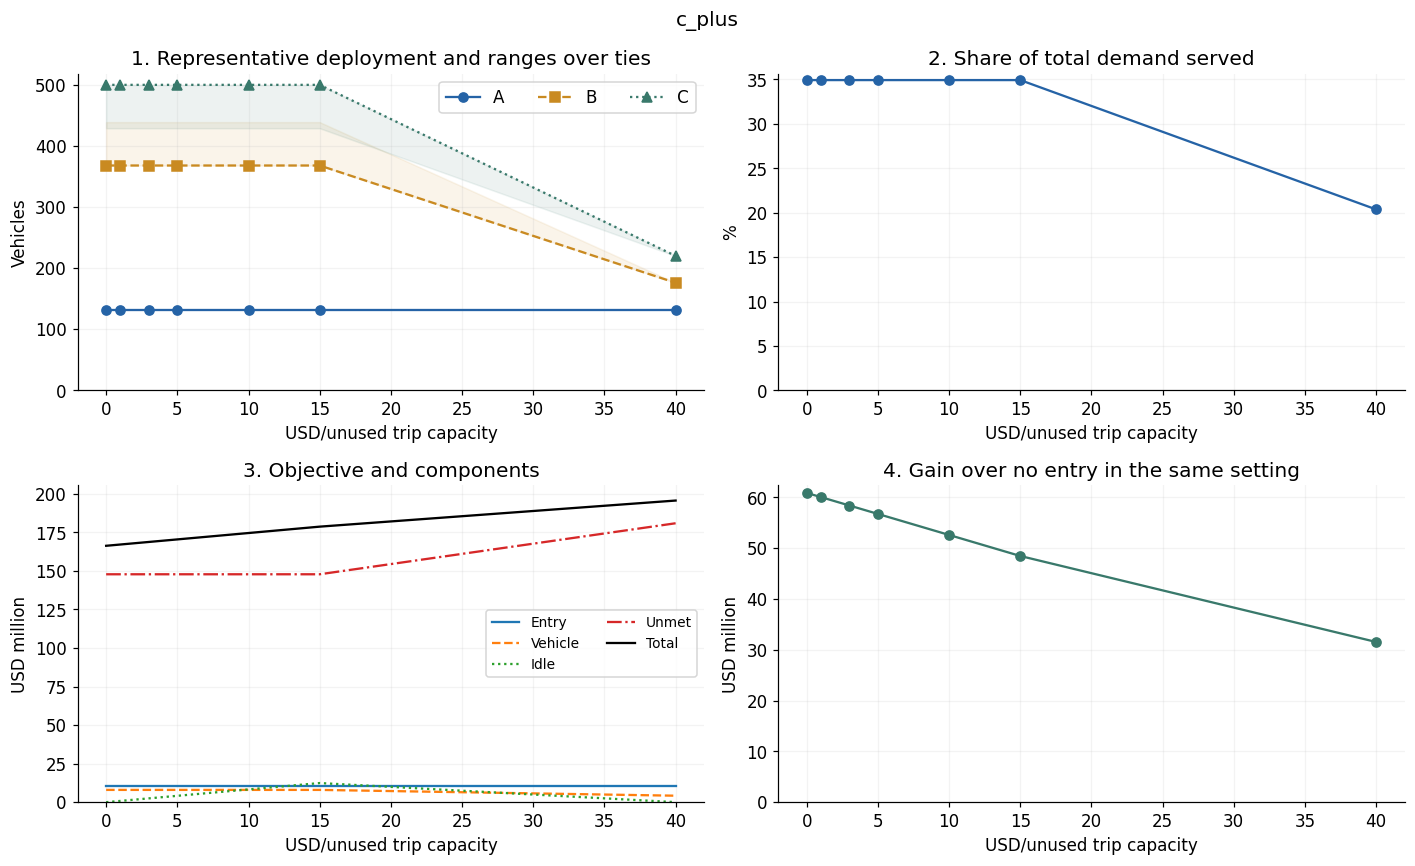
\includegraphics[width=\linewidth]{figures/annual/sweep_c_plus.png}
\caption{Sensitivity of allocations and performance to the unused-capacity penalty.}\label{fig:an-sweep_cplus}
\end{figure}
\textbf{Interpretation.} From 0 to 15 the allocation is unchanged and $Z=166{,}263{,}859+827{,}397\,c^+$, the baseline objective plus the penalty on the baseline's average unused capacity.
The penalty does not reorder cities because it lowers the value of every partially used vehicle in the same way, and the fleet limit keeps all 1{,}000 vehicles in use.
It changes the decision only when a vehicle's value turns negative. A vehicle on the 62{,}108 step idles $8{,}760\times0.2=1{,}752$ trips per year on average, so its value is $62{,}108-1{,}752\,c^+$, which reaches zero at $c^+\approx35.4$.
At $c^+=40$ the fleet shrinks to $(132,176,220)$, exactly the 528 vehicles that are used in every scenario.
The penalty can also be absorbed into the other cost parameters: because $O_c^s=\kappa_cq_c-D_c^s+U_c^s$, the objective with $(K_c,c_c^-,c_c^+)$ equals the objective with $(K_c+c_c^+\kappa_c,\;c_c^-+c_c^+,\;0)$ up to a constant, so $c^+$ is not an independent decision lever.

\clearpage
\subsubsection{Forgone Contribution Margin $c^-$}
\begin{table}[H]
\centering\small
\caption{Selected Results: Common Forgone Contribution Margin}\label{tab:an-selected-cminus}
\begin{tabular}{lrrrrrr}
\toprule
Value & $q^{\mathrm{rep}}$ & Ties & $\bar T$ & $\mathrm{SR}$ (\%) & $Z$ & $\Delta Z$\\\midrule
2 & $(0,0,500)$ & 1 & 3,889,272 & 17.12 & 45.13 & 0.29\\
5 & $(0,500,500)$ & 1 & 7,543,306 & 33.21 & 90.81 & 22.74\\
10 & $(132,368,500)$ & 72 & 7,932,603 & 34.93 & 166.26 & 60.85\\
15 & $(132,368,500)$ & 72 & 7,932,603 & 34.93 & 240.16 & 100.52\\
20 & $(132,368,500)$ & 72 & 7,932,603 & 34.93 & 314.06 & 140.18\\
\bottomrule
\end{tabular}
\end{table}
\begin{figure}[H]
\centering
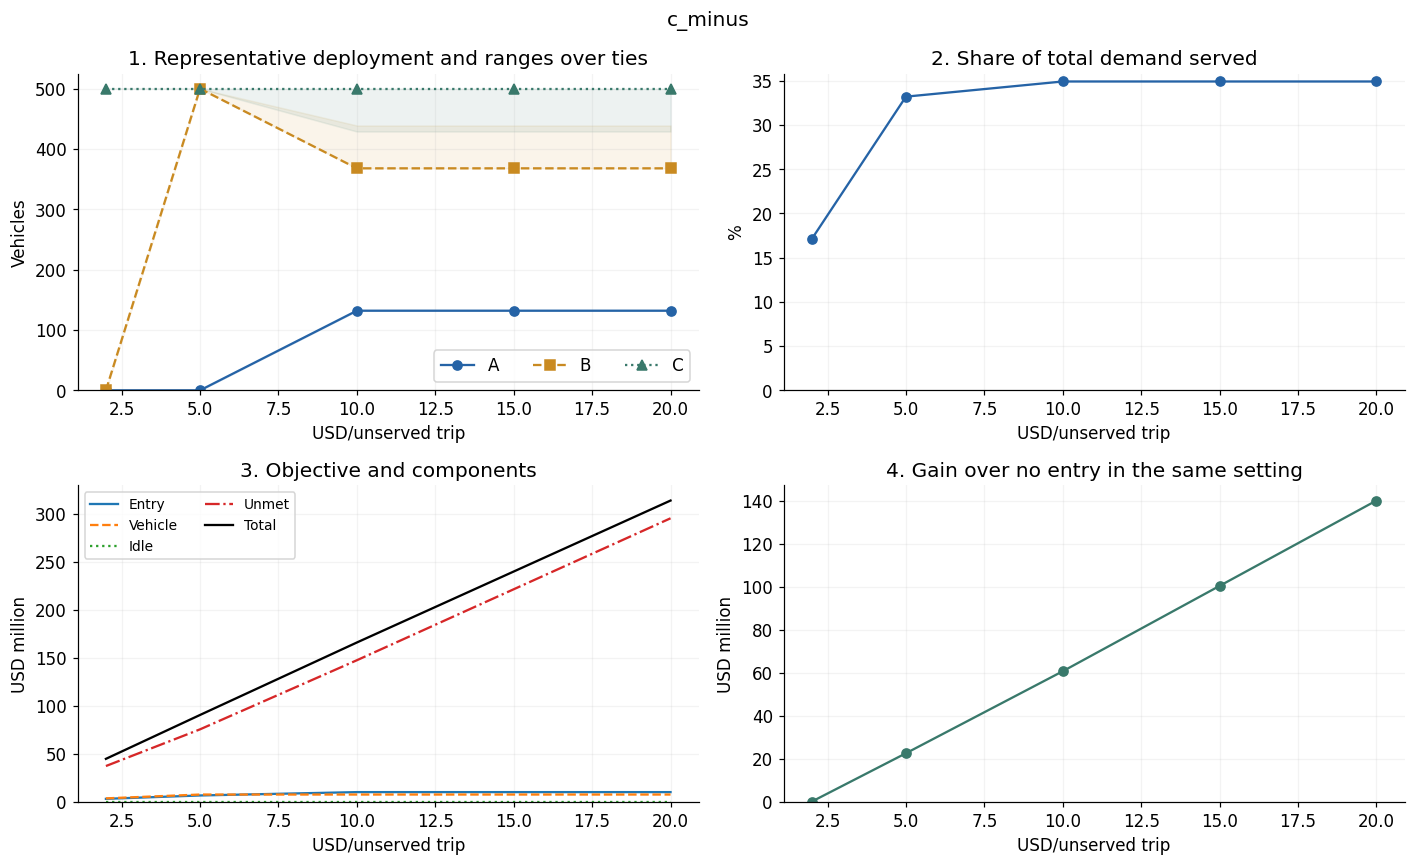
\includegraphics[width=\linewidth]{figures/annual/sweep_c_minus.png}
\caption{Results from varying the forgone contribution margin.}\label{fig:an-sweep_cminus}
\end{figure}
\textbf{Interpretation.} The margin decides how many entry costs are worth paying. At $c^-=2$ a vehicle used in every scenario earns $8{,}760\times2-7{,}972=9{,}548$, and only C's 500 vehicles recover an entry cost; at 5 two cities are entered; from 10 upward all three. Above 10 the allocation is fixed and $\Delta Z$ grows linearly.

\clearpage
\subsubsection{Market Size of A: $M_A$}
\begin{table}[H]
\centering\small
\caption{Selected Results: A's Market-Size Multiplier}\label{tab:an-selected-MA}
\begin{tabular}{lrrrrrr}
\toprule
Value & $q^{\mathrm{rep}}$ & Ties & $\bar T$ & $\mathrm{SR}$ (\%) & $Z$ & $\Delta Z$\\\midrule
0.7500 & $(0,500,500)$ & 1 & 7,543,306 & 35.37 & 152.79 & 60.46\\
0.8125 & $(0,500,500)$ & 1 & 7,543,306 & 34.81 & 156.25 & 60.46\\
0.8750 & $(116,384,500)$ & 56 & 7,903,275 & 35.89 & 159.62 & 60.56\\
0.9375 & $(124,376,500)$ & 64 & 7,917,939 & 35.40 & 162.94 & 60.71\\
1.0000 & $(132,368,500)$ & 72 & 7,932,603 & 34.93 & 166.26 & 60.85\\
1.0625 & $(140,360,500)$ & 80 & 7,946,770 & 34.46 & 169.59 & 61.00\\
1.1250 & $(149,351,500)$ & 89 & 7,961,054 & 34.01 & 172.91 & 61.14\\
1.1875 & $(157,343,500)$ & 97 & 7,975,717 & 33.58 & 176.24 & 61.29\\
1.2500 & $(165,335,500)$ & 105 & 7,990,381 & 33.16 & 179.56 & 61.43\\
\bottomrule
\end{tabular}
\end{table}
\begin{figure}[H]
\centering
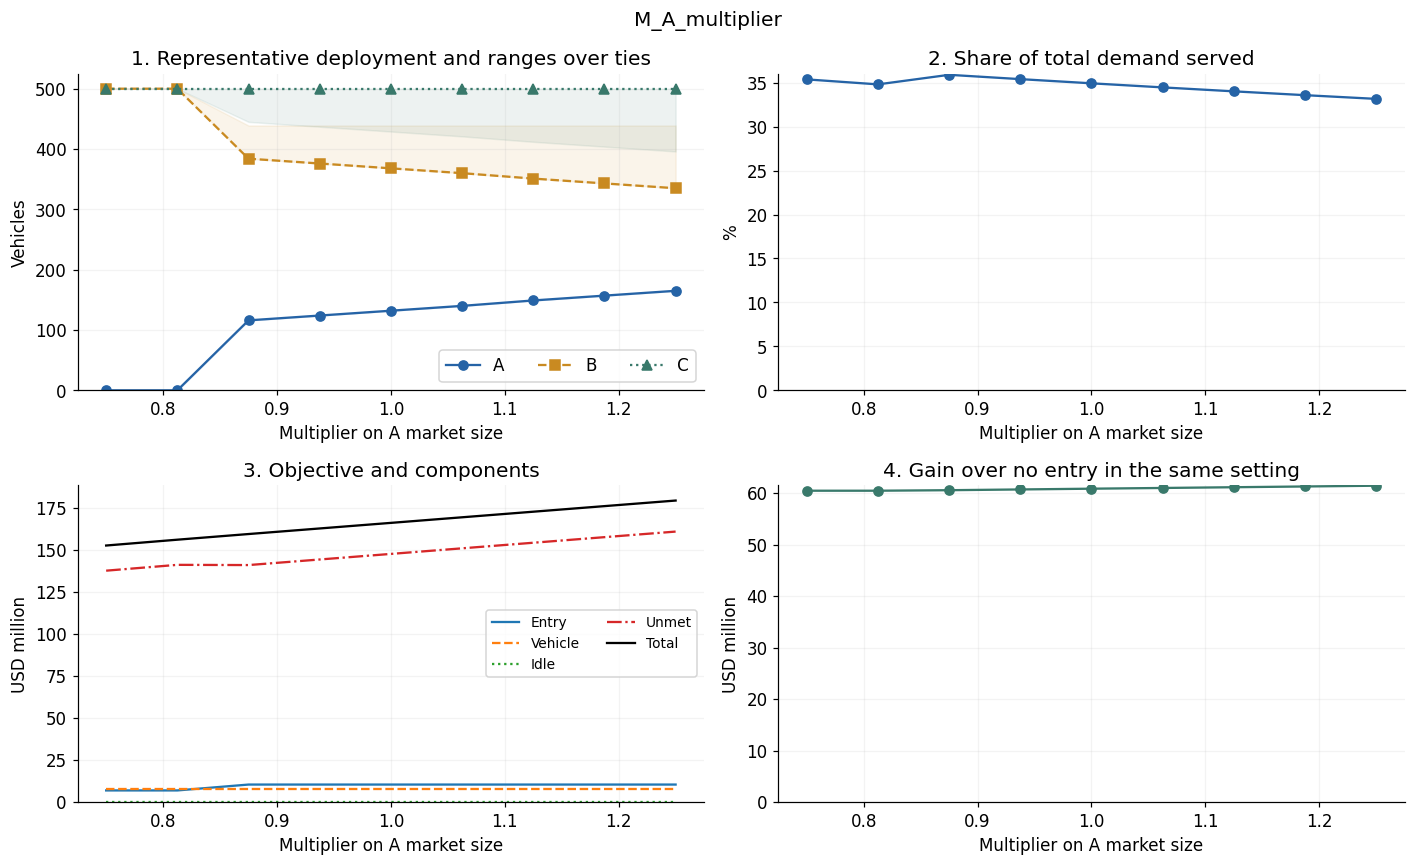
\includegraphics[width=\linewidth]{figures/annual/sweep_M_A_multiplier.png}
\caption{Results from varying only A's market size. A multiplier of 1 corresponds to $M_A=577{,}908{,}105$.}\label{fig:an-sweep_MA}
\end{figure}
\textbf{Interpretation.} A's fleet follows its smallest demand scenario: the 132 always-used slots become 116 at $0.875$ and 165 at $1.25$, and the vehicles come from B. Below $0.875$ the always-used slots are too few to repay the entry cost and A is not entered.

\clearpage
\subsubsection{Demand Variability $\alpha$ with Fixed Mean Demand}
\begin{table}[H]
\centering\small
\caption{Selected Results: Demand Variability}\label{tab:an-selected-alpha}
\begin{tabular}{lrrrrrr}
\toprule
Value & $q^{\mathrm{rep}}$ & Ties & $\bar T$ & $\mathrm{SR}$ (\%) & $Z$ & $\Delta Z$\\\midrule
0.0 & $(0,500,500)$ & 3 & 8,760,000 & 38.57 & 154.49 & 72.63\\
0.2 & $(0,500,500)$ & 3 & 8,760,000 & 38.57 & 154.49 & 72.63\\
0.3 & $(0,500,500)$ & 1 & 8,760,000 & 38.57 & 154.49 & 72.63\\
0.5 & $(0,500,500)$ & 1 & 8,760,000 & 38.57 & 154.49 & 72.63\\
0.6 & $(0,500,500)$ & 1 & 8,679,202 & 38.21 & 155.30 & 71.82\\
0.7 & $(0,500,500)$ & 1 & 8,523,275 & 37.53 & 156.86 & 70.26\\
0.8 & $(232,315,453)$ & 60 & 8,655,811 & 38.11 & 159.03 & 68.09\\
0.9 & $(182,318,500)$ & 165 & 8,294,282 & 36.52 & 162.65 & 64.47\\
1.0 & $(132,368,500)$ & 72 & 7,932,603 & 34.93 & 166.26 & 60.85\\
\bottomrule
\end{tabular}
\end{table}
\begin{figure}[H]
\centering
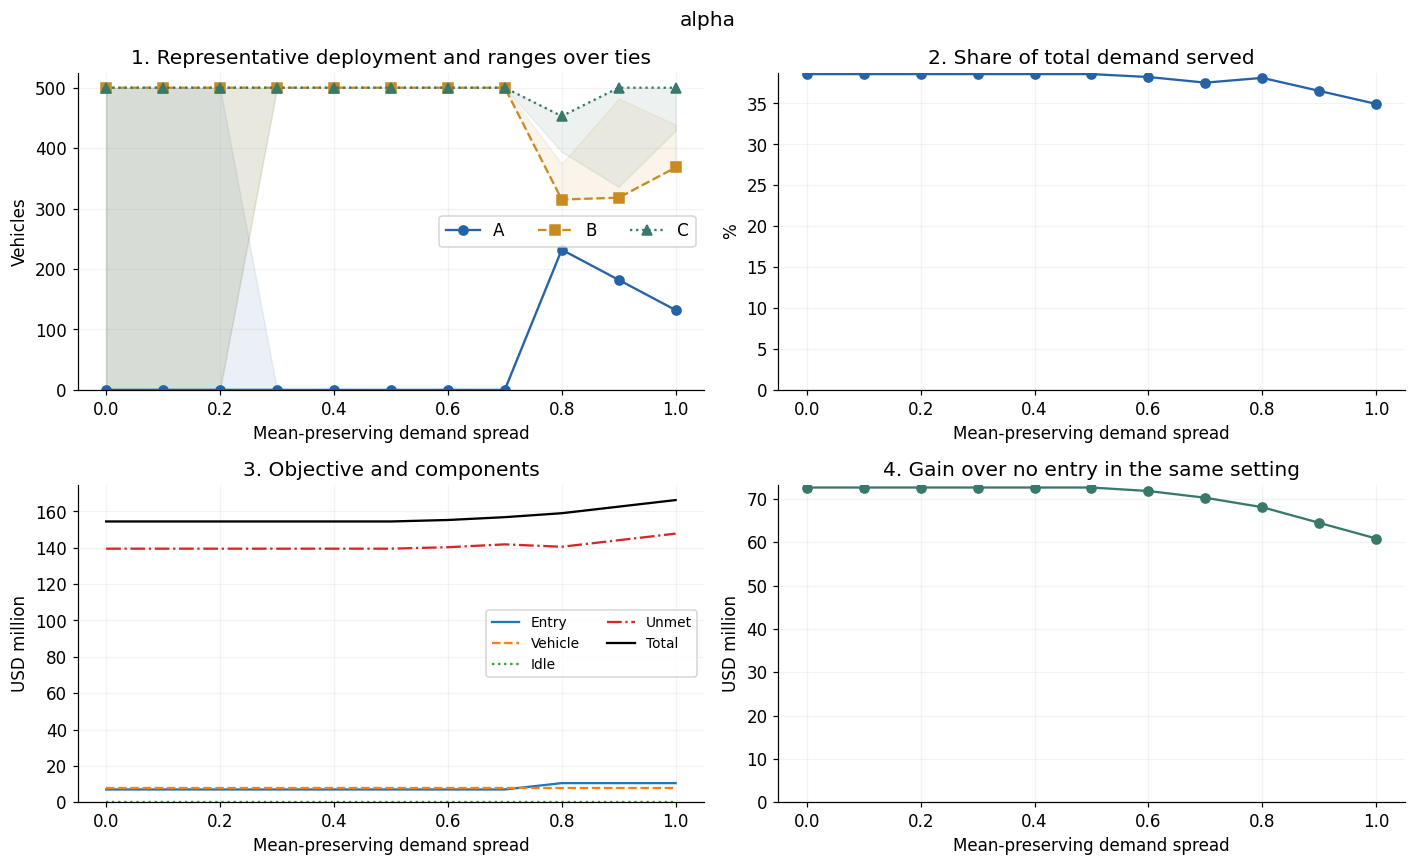
\includegraphics[width=\linewidth]{figures/annual/sweep_alpha.png}
\caption{Results from varying demand variability while preserving mean demand.}\label{fig:an-sweep_alpha}
\end{figure}
\textbf{Interpretation.} With little variability every scenario demand exceeds 500 vehicles' capacity, so two cities with 500 vehicles each are optimal and, up to $\alpha=0.2$, any two cities tie.
As variability grows, low-demand scenarios appear in B and C, their late vehicles lose value, and from $\alpha=0.8$ the fleet spreads to A. The improvement falls from 72.63 to 60.85 million: variability costs money even when the mean is unchanged.

\FloatBarrier
\subsection{City-Specific Changes, One at a Time}\label{sec:an-city}
Each cell changes the listed input in one city only and reports the representative allocation, the number of tied optima in parentheses, and $\Delta Z$ in USD million. The baseline is $(132,368,500)$ (72) with $\Delta Z=60.85$.
\begin{table}[H]
\centering\footnotesize
\caption{One-City Changes: Representative Allocation (Ties); $\Delta Z$ in USD Million}\label{tab:an-city}
\begin{tabular}{lP{.27\linewidth}P{.27\linewidth}P{.27\linewidth}}
\toprule
Change & In A & In B & In C\\\midrule
$M_c\times0.75$ & $(0,500,500)$ (1); 60.46 & $(170,330,500)$ (1); 59.75 & $(132,440,428)$ (16); 59.75\\
$M_c\times1.25$ & $(165,335,500)$ (105); 61.43 & $(0,500,500)$ (1); 62.81 & $(132,368,500)$ (72); 61.82\\
$p_c^s\times0.75$ & $(0,500,500)$ (1); 60.46 & $(170,330,500)$ (1); 59.75 & $(132,440,428)$ (16); 59.75\\
$p_c^s\times1.25$ & $(165,335,500)$ (105); 61.43 & $(0,500,500)$ (1); 62.81 & $(132,368,500)$ (72); 61.82\\
$\kappa_c\times0.75$ & $(0,500,500)$ (1); 60.46 & $(266,234,500)$ (1); 55.57 & $(267,440,293)$ (1); 54.53\\
$\kappa_c\times1.25$ & $(264,236,500)$ (204); 63.74 & $(148,352,500)$ (1); 66.88 & $(132,368,500)$ (1); 68.95\\
$F_c\times0.75$ & $(132,368,500)$ (72); 61.73 & $(132,368,500)$ (72); 61.73 & $(132,368,500)$ (72); 61.73\\
$F_c\times1.25$ & $(0,500,500)$ (1); 60.46 & $(132,368,500)$ (72); 59.98 & $(132,368,500)$ (72); 59.98\\
$K_c\times0.75$ & $(132,368,500)$ (72); 61.12 & $(132,439,429)$ (1); 61.73 & $(132,368,500)$ (1); 61.85\\
$K_c\times1.25$ & $(132,368,500)$ (72); 60.59 & $(132,368,500)$ (1); 60.12 & $(132,439,429)$ (1); 60.00\\
$c_c^-\times0.75$ & $(0,500,500)$ (1); 60.46 & $(324,176,500)$ (1); 55.32 & $(330,440,230)$ (1); 54.12\\
$c_c^-\times1.25$ & $(330,176,494)$ (264); 65.04 & $(0,500,500)$ (1); 69.60 & $(132,368,500)$ (1); 70.58\\
$c_c^+=1$ & $(132,368,500)$ (72); 60.85 & $(132,368,500)$ (1); 60.52 & $(132,439,429)$ (1); 60.49\\
$c_c^+=3$ & $(132,368,500)$ (72); 60.85 & $(132,368,500)$ (1); 59.84 & $(132,440,428)$ (1); 59.76\\
$c_c^+=5$ & $(132,368,500)$ (72); 60.85 & $(132,368,500)$ (193); 59.17 & $(132,440,428)$ (198); 59.03\\
$\bar q_c=100$ & $(0,500,500)$ (1); 60.46 & $(400,100,500)$ (1); 55.95 & $(400,500,100)$ (61); 53.59\\
$\bar q_c=1{,}000$ & $(132,368,500)$ (72); 60.85 & $(132,368,500)$ (72); 60.85 & $(0,440,560)$ (1); 61.95\\
\bottomrule
\end{tabular}
\end{table}
\begin{figure}[H]
\centering
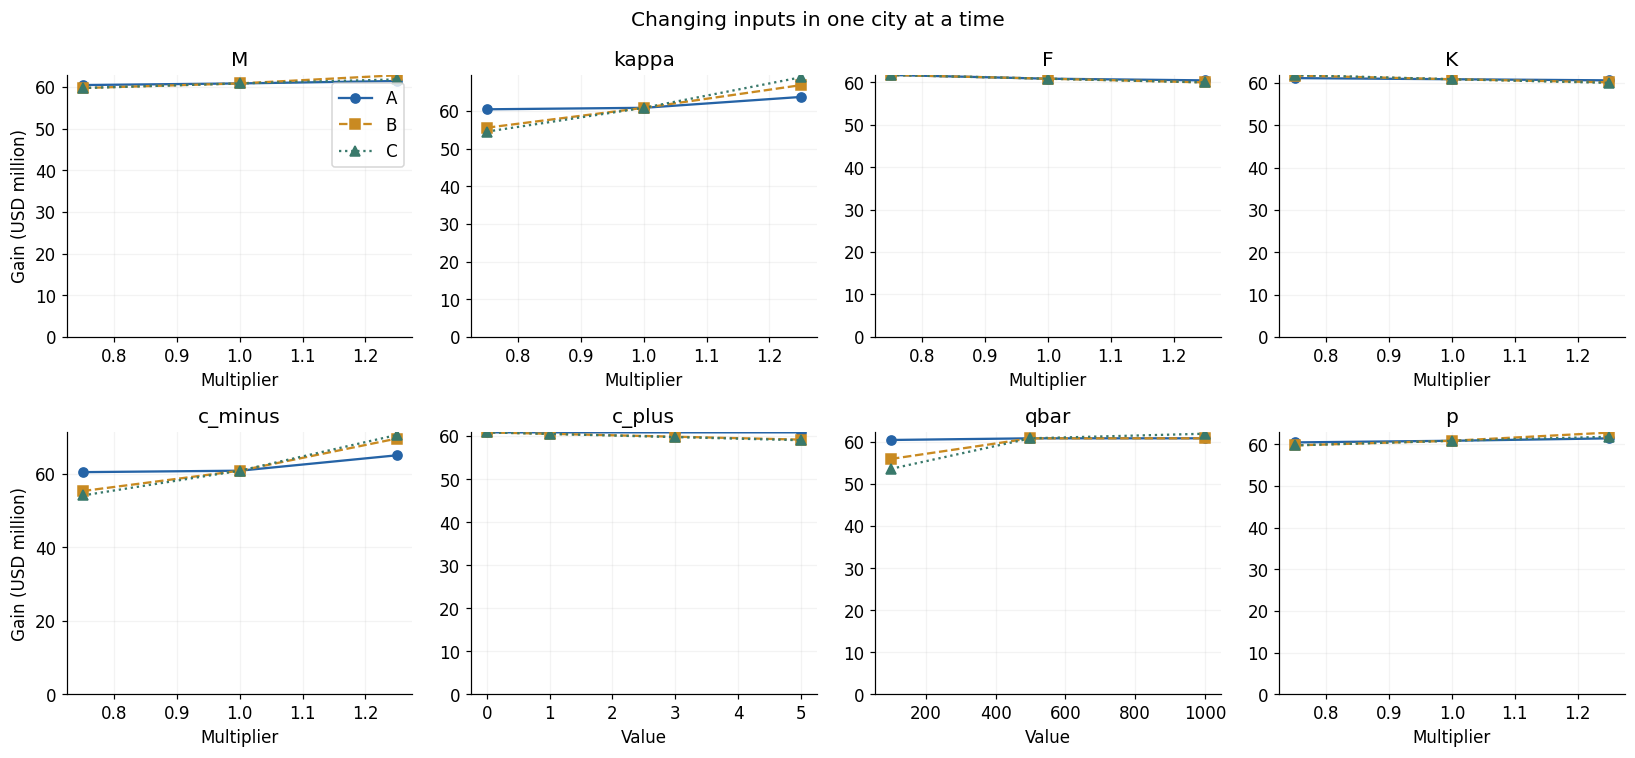
\includegraphics[width=\linewidth]{figures/annual/15_city_sensitivity.png}
\caption{Improvement over no entry when one input is changed in one city.}\label{fig:an-15_city}
\end{figure}
\textbf{Interpretation.} A cheaper or more productive city attracts vehicles: lower $F$ or $K$, or higher $\kappa$ or $c^-$, in one city pulls the fleet toward it, and the opposite change pushes the fleet away.
Unlike the reference-level run, one city's $M$ or $p$ now matters too: a 25\% larger market in B removes A, while a 25\% smaller market in C moves vehicles from C to B.
Small city-specific costs act as tie breakers: an unused-capacity penalty of 1 in B alone makes $(132,368,500)$ the unique optimum, and the same penalty in C alone selects $(132,439,429)$, because idle capacity now costs money in one city only.
A common change that leaves the allocation unchanged therefore says nothing about robustness to differences between cities.

\FloatBarrier
\subsection{Summary}
\begin{table}[H]
\centering\small
\caption{Where the Optimal Allocation Changes (Baseline $(132,368,500)$)}\label{tab:an-summary}
\begin{tabular}{lP{.30\linewidth}P{.44\linewidth}}
\toprule
Input & Range examined & Allocation change\\\midrule
$Q$ & 0--2{,}000 & C only up to 500; B added at 600; A added at 1{,}000; limits bind at 1{,}500\\
$F$ (common) & $\pm25\%$ & A dropped above $3{,}892{,}967$\\
$K$ (common) & $\pm25\%$ & None; $\Delta Z$ changes linearly\\
$\kappa$ (common) & $\pm25\%$ & A dropped at $\le8{,}212.5$ (switch near 8{,}498)\\
$M$ or $p$ (common) & $\times0.75$--$1.25$ & A dropped at $\ge1.0625$ (switch near 1.042); more vehicles in A when demand is smaller\\
$\bar q$ & 100--1{,}500 & Even split at 100, 250; $(0,440,560)$ from 750\\
$c^+$ (common) & 0--40 & None up to 15; fleet shrinks to 528 at 40 (switch near 35.4)\\
$c^-$ (common) & 2--20 & One city at 2, two at 5, three from 10\\
$M_A$ & $\times0.75$--$1.25$ & A dropped at $\le0.8125$; $q_A$ from 116 to 165 otherwise\\
$\alpha$ & 0--1 & Two cities up to 0.7; three cities from 0.8\\
One-city changes & $\pm25\%$; $c^+$ 1--5; $\bar q$ 100, 1{,}000 & Vehicles move toward the cheaper or more productive city; single-city $c^+$ breaks the B--C tie\\
\bottomrule
\end{tabular}
\end{table}
Three points carry over to the modeling discussion. First, city-specific demand differences affect the allocation only when demand and capacity are of the same order; when demand dominates, cost parameters alone decide.
Second, with ten equally likely scenarios and $c^+=0$ the value of a vehicle is a step function, which produces large sets of tied optima; more scenarios or a positive $c^+$ reduce them.
Third, the switching points reported here belong to this synthetic instance and are not estimates for real cities.

\end{document}
